\section{} % Question 1

% Code
\begin{minted}[mathescape, linenos, numbersep=5pt, frame=lines, framesep=2mm, tabsize=4, numberblanklines=true, breaklines=true]{matlab}
>> test
percentage of ones: 73.41%
percentage of twos: 26.59%
\end{minted}


\begin{figure}[H]
	\centering
	\begin{minipage}{.45\textwidth}
		\centering
		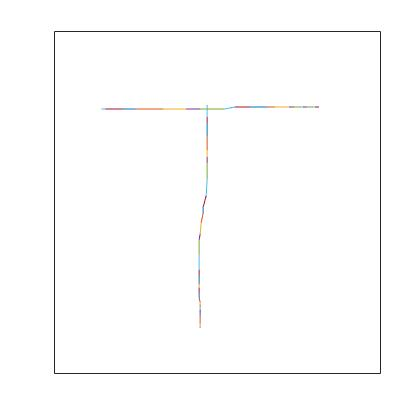
\includegraphics[width=.7\linewidth]{images/T_drawing}
		\captionof{figure}{Drawing of capital T (first line down, then line to right)}
		\label{fig:features_T}
	\end{minipage}%
	\begin{minipage}{.45\textwidth}
		\centering
		\includegraphics[width=.99\linewidth]{images/T_bar}
		\captionof{figure}{Extracted features, 1 is line down, 2 is line to the right}
		\label{fig:features_plus}
	\end{minipage}
\end{figure}
\begin{figure}[H]
	\centering
	\begin{minipage}{.45\textwidth}
		\centering
		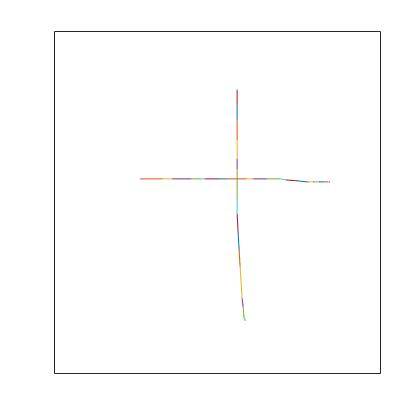
\includegraphics[width=.7\linewidth]{images/+_drawing}
		\captionof{figure}{Features of + sign (first line down, then line to right)}
		\label{fig:features_T}
	\end{minipage}%
	\begin{minipage}{.45\textwidth}
		\centering
		\includegraphics[width=.99\linewidth]{images/+_bar}
		\captionof{figure}{Extracted features, 1 is line down, 2 is line to the right}
		\label{fig:features_plus}
	\end{minipage}
\end{figure}